\documentclass[10pt]{article}
\usepackage[margin=0.9in]{geometry}
\usepackage{graphicx}
\usepackage{booktabs}
\usepackage{amsmath}
\usepackage{float}
\usepackage[hidelinks]{hyperref}
\usepackage{caption}
\graphicspath{{figures/}}

\title{What Post-Training Changes: Reasoning Gains and Safety Side Effects of ES vs RL}
\author{Jaysen Ma}
\date{}

\begin{document}
\maketitle

\begin{abstract}
Recent work post-trains large language models to improve maths, programming and other skills. Reinforcement learning with verifiable rewards (RLVR), usually via GRPO, is the common method, and evolution strategies (ES) are being studied as an alternative. We ask what these post-training methods change beyond the target metric, on two axes: reasoning capacity, measured by pass@$k$, and moral judgement, measured on ETHICS. We compare Qwen2.5-1.5B and Qwen2.5-7B base models with ES and GRPO arms trained on the same 8,523 maths problems (the GRPO arms are the public SimpleRL-Zoo checkpoints), scoring pass@$k$ up to 512 on four benchmarks. At 1.5B both methods stay above base at every measured $k$. At 7B, GRPO leads at small $k$ but falls below base as $k$ grows on all four benchmarks, while ES finishes at or above base on three of four. Neither method changes MMLU accuracy. On the ETHICS commonsense subset, however, 7B ES lowers accuracy from 63.42\% to 57.68\% (paired McNemar test, $p = 9\times10^{-34}$), while 7B GRPO is unchanged and MMLU shows no change for the same checkpoint. All results are one run per method and not compute-matched.
\end{abstract}

\begin{figure}[h]\centering
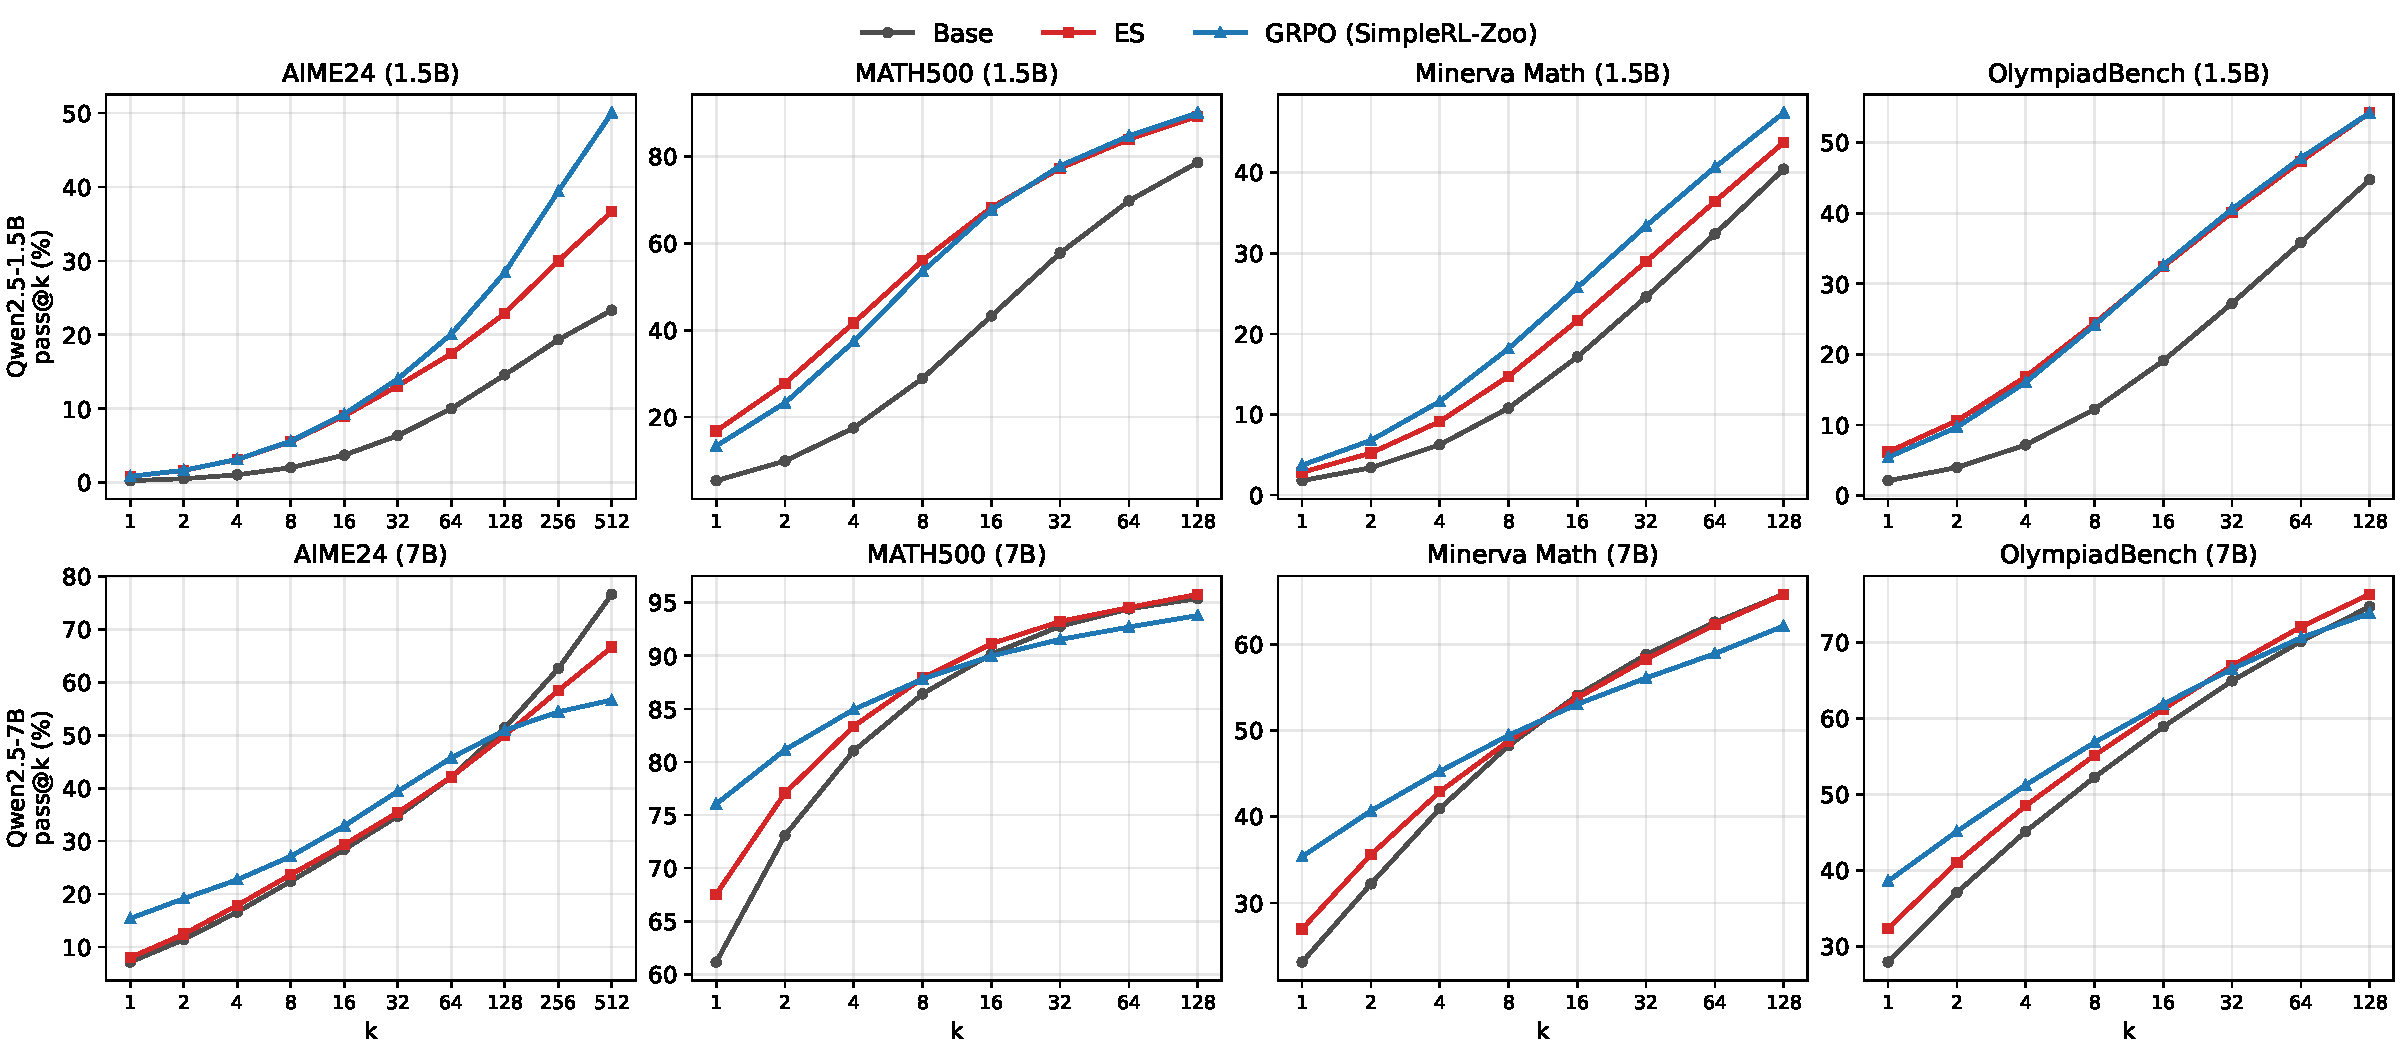
\includegraphics[width=\linewidth]{hero_passk.pdf}
\caption{pass@$k$ (the chance that at least one of $k$ sampled answers is correct) of the base model, ES and GRPO (SimpleRL-Zoo) on AIME24, MATH500, Minerva Math and OlympiadBench. Top: Qwen2.5-1.5B, where ES and GRPO stay above base at every $k$ on all four benchmarks. Bottom: Qwen2.5-7B, where GRPO leads at small $k$ but the base finishes above it on all four benchmarks, while ES finishes at or above base on three of four.}\label{fig:hero}
\end{figure}

\section{Introduction}
Recent work post-trains large language models on tasks with checkable answers to improve maths, programming and other skills. The common method is reinforcement learning with verifiable rewards (RLVR), usually GRPO (group relative policy optimisation), which samples several answers per prompt and uses their relative rewards as the learning signal; SimpleRL-Zoo~\cite{simplerl} applies it to open base models. Evolution strategies (ES) are being studied as an alternative~\cite{qiu}: ES perturbs all parameters with random noise, scores a population of perturbed models, and moves towards the better ones, without backpropagation.

Both methods are judged mainly by the metric they target, such as pass@1 on a maths benchmark. We ask what else they change, comparing ES and GRPO trained on the same task, reward and data, on two axes. The first is \emph{reasoning capacity}, measured by pass@$k$: the probability that at least one of $k$ sampled answers is correct. pass@1 measures how often a single sample is right; pass@$k$ at large $k$ measures which problems the model can solve at all. Yue et al.~\cite{yue} motivate this lens: they show that RLVR tends to narrow the large-$k$ ceiling, so that the trained model wins at small $k$ but the base model overtakes it as $k$ grows. We ask whether the same holds for each method here.

The second axis is \emph{moral judgement}. All post-training here is maths-only, so any change outside maths is something nobody trained for. Standard forgetting checks such as MMLU measure capability. We additionally ask whether maths-only post-training shifts moral judgements, as measured by ETHICS~\cite{ethics}, in ways those capability checks do not detect.

Our findings, in the order of the sections below:
\begin{enumerate}
\item At 1.5B, neither ES nor GRPO narrows the pass@$k$ ceiling: both stay above base at every measured $k$.
\item At 7B, GRPO leads at small $k$ but falls below base as $k$ grows on all four benchmarks, whereas ES finishes at or above base on three of four (Figure~\ref{fig:hero}).
\item Neither method changes MMLU accuracy at either scale, although ES moves the weights far more than GRPO.
\item Capability and moral judgement can move separately. Despite unchanged MMLU accuracy, 7B-ES lowers ETHICS commonsense accuracy while 7B-GRPO does not. A post-training method can preserve or improve capability while shifting moral judgements, and a capability check alone can miss the shift.
\end{enumerate}

\section{Setup}
\paragraph{Models and arms.} We use two base models, \texttt{Qwen2.5-1.5B} and \texttt{Qwen2.5-7B}, and compare each with two post-trained arms. We name the six models 1.5B-Base, 1.5B-ES, 1.5B-GRPO, 7B-Base, 7B-ES and 7B-GRPO.

\paragraph{ES arm.} We trained full-parameter ES with Qiu et al.'s method and code~\cite{qiu}, using identical hyperparameters at both scales: noise scale $\sigma = 0.001$, learning rate $\alpha = \sigma/2 = 0.0005$, population 32, 50 iterations, batch 256, 2,048-token cap. The training data were the 8,523 level-3-to-5 MATH problems used by SimpleRL-Zoo, in the same order. Each run used 8$\times$ RTX 4090 48GB and took 3h22m (1.5B) or 4h35m (7B).

\paragraph{GRPO arm.} We use the published SimpleRL-Zoo GRPO checkpoint~\cite{simplerl} at each scale. It was trained on the same problems with a much larger budget (Table~\ref{tab:budget}).

\begin{table}[H]\centering\small
\begin{tabular}{lccccccc}\toprule
 & Prompts/step & Steps & Samples per prompt & Prompt visits & Epochs & Generations & Token cap\\\midrule
ES & 256 & 50 & 32 (population) & 12,800 & 1.50 & 409,600 & 2,048\\
GRPO & 1,024 & $\sim$100 & 8 (rollouts) & 102,400 & 12.01 & 819,200 & 8,192\\
GRPO/ES & 4$\times$ & 2$\times$ & 0.25$\times$ & 8$\times$ & 8$\times$ & 2$\times$ & 4$\times$\\\bottomrule
\end{tabular}
\caption{Training budgets. Prompt visits = prompts/step $\times$ steps. GRPO sees 8$\times$ more data but only 2$\times$ more generations. The 7B GRPO checkpoint took $\sim$15h on 2 nodes of 8$\times$ H100.}
\label{tab:budget}
\end{table}

\paragraph{Benchmarks and metrics.} We evaluate on AIME24 ($n=30$, $k\le512$), MATH500 ($n=500$), Minerva Math ($n=272$) and OlympiadBench ($n=675$), the last three with $k\le128$. Generation settings were identical throughout: temperature 0.6, top-$p$ 0.95, 2,048 max tokens, the Qwen prompt template that asks for a \verb|\boxed{}| answer, seed 1. \emph{pass@max} is pass@$k$ at the largest $k$ sampled. We also report a per-question breakdown: a question is \emph{solvable} if at least one of the samples is correct; \emph{narrow} is the share of questions the base solves and the trained model does not, \emph{gain} the reverse, and \emph{net coverage} = gain $-$ narrow.

\paragraph{Grader.} The pass@$k$ evaluation extracts answers with the Qwen2.5-Math toolkit parser (\verb|\boxed{}|, then ``the answer is'', then ``final answer is'', then the last number), the same rule SimpleRL-Zoo trained against. ES was rewarded only for the last \verb|\boxed{}|. ES raised \verb|\boxed{}| emission from 14.6\% to 24.2\%, a gain the lenient evaluation largely ignores; this grader therefore probably favours GRPO over ES.

\paragraph{Statistics.} Every model answers the same items, so we compare each trained arm with its own base using a paired (exact McNemar) test: it ignores items both get right or both get wrong, and asks whether the trained arm's wins among the disagreements differ from a coin flip. Within each benchmark family we correct for multiple comparisons with Bonferroni: for MMLU (4 comparisons) we report $p$ multiplied by 4; for ETHICS (20 comparisons) we report raw $p$ and call a change significant if $p < 0.05/20 = 0.0025$. Both amount to the same family-wise 0.05 criterion.

\section{Reasoning results}
We first ask whether each trained model keeps its base model's pass@$k$ ceiling. Figure~\ref{fig:hero} shows the pass@$k$ curves; Tables~\ref{tab:passk} and \ref{tab:solv} summarise them.

\begin{table}[H]\centering\small
\setlength{\tabcolsep}{4pt}
\begin{tabular}{llcccccc}\toprule
 & & \multicolumn{3}{c}{Qwen2.5-1.5B} & \multicolumn{3}{c}{Qwen2.5-7B}\\\cmidrule(lr){3-5}\cmidrule(lr){6-8}
Benchmark & Metric & Base & ES & GRPO & Base & ES & GRPO\\\midrule
AIME24 & pass@1 & 0.28 & 0.87 & 0.87 & 7.14 & 7.98 & 15.39\\
 & pass@max & 23.33 & 36.67 & 50.00 & 76.67 & 66.67 & 56.67\\
MATH500 & pass@1 & 5.37 & 16.79 & 13.35 & 61.15 & 67.54 & 76.04\\
 & pass@max & 78.60 & 89.20 & 90.00 & 95.40 & 95.80 & 93.80\\
Minerva & pass@1 & 1.79 & 2.83 & 3.72 & 23.14 & 26.99 & 35.38\\
 & pass@max & 40.44 & 43.75 & 47.43 & 65.81 & 65.81 & 62.13\\
OlympiadBench & pass@1 & 2.10 & 6.17 & 5.41 & 27.95 & 32.39 & 38.59\\
 & pass@max & 44.74 & 54.22 & 54.22 & 74.67 & 76.30 & 73.78\\\bottomrule
\end{tabular}
\caption{pass@1 and pass@max (\%). pass@max is $k=512$ for AIME24 and $k=128$ otherwise.}\label{tab:passk}
\end{table}

\begin{table}[H]\centering\small
\setlength{\tabcolsep}{4pt}
\begin{tabular}{lcccccccccccc}\toprule
 & \multicolumn{3}{c}{1.5B-ES} & \multicolumn{3}{c}{1.5B-GRPO} & \multicolumn{3}{c}{7B-ES} & \multicolumn{3}{c}{7B-GRPO}\\
\cmidrule(lr){2-4}\cmidrule(lr){5-7}\cmidrule(lr){8-10}\cmidrule(lr){11-13}
Benchmark & narrow & gain & net & narrow & gain & net & narrow & gain & net & narrow & gain & net\\\midrule
AIME24 & 0.0 & 13.3 & +13.3 & 3.3 & 30.0 & +26.7 & 13.3 & 3.3 & $-$10.0 & 23.3 & 3.3 & $-$20.0\\
MATH500 & 1.4 & 12.0 & +10.6 & 1.2 & 12.6 & +11.4 & 1.0 & 1.4 & +0.4 & 3.0 & 1.4 & $-$1.6\\
Minerva & 7.0 & 10.3 & +3.3 & 5.5 & 12.5 & +7.0 & 2.9 & 2.9 & 0.0 & 5.1 & 1.5 & $-$3.6\\
OlympiadBench & 3.9 & 13.3 & +9.4 & 3.4 & 12.9 & +9.5 & 3.4 & 5.0 & +1.6 & 5.5 & 4.6 & $-$0.9\\\bottomrule
\end{tabular}
\caption{Solvable-question breakdown vs.\ own base, \% of questions; net coverage = gain $-$ narrow.}\label{tab:solv}
\end{table}

\paragraph{1.5B.} Neither method narrows the ceiling. 1.5B-ES and 1.5B-GRPO stay above base at every measured $k$ on all four benchmarks, with no crossover, and both expand question coverage on all four. 1.5B-ES tracks 1.5B-GRPO at pass@16 on three of four benchmarks (AIME24 9.04 vs.\ 9.27\%, MATH500 68.24 vs.\ 67.70\%, OlympiadBench 32.43 vs.\ 32.64\%; Minerva 21.65 vs.\ 25.74\%) with $\sim$1/8 of the data budget.

\paragraph{7B.} At 7B the two methods diverge. 7B-GRPO leads the base at small $k$: up to $k=64$ on AIME24 and OlympiadBench and up to $k=8$ on MATH500 and Minerva. Beyond that it falls below base, finishing below on all four benchmarks (net coverage $-20.0$ points on AIME24). 7B-ES improves pass@1 slightly; it finishes at or above base on MATH500, Minerva and OlympiadBench, and falls below base on AIME24 from $k=128$ (net coverage $-10.0$).

\paragraph{Interpretation.} These results suggest that ES preserves the ceiling better than GRPO at 7B. Budget and grader both confound the comparison (Section~\ref{sec:lim}): ES ran 50 iterations, a tenth of the 500 that Qiu et al.\ suggest, against a GRPO checkpoint that saw 8$\times$ the data.

\section{How far did the weights move?}
Before testing for side effects, we measure how much each method changes the model. For every parameter we take the trained value minus the base value. ES moves the weights much further than GRPO: by standard deviation of the differences, 56$\times$ at 1.5B and 74$\times$ at 7B (at 7B, $\sigma = 6.8\times10^{-4}$ for ES vs.\ $9.2\times10^{-6}$ for GRPO). GRPO makes a far smaller and more selective change (Figure~\ref{fig:w}).

\begin{figure}[H]\centering
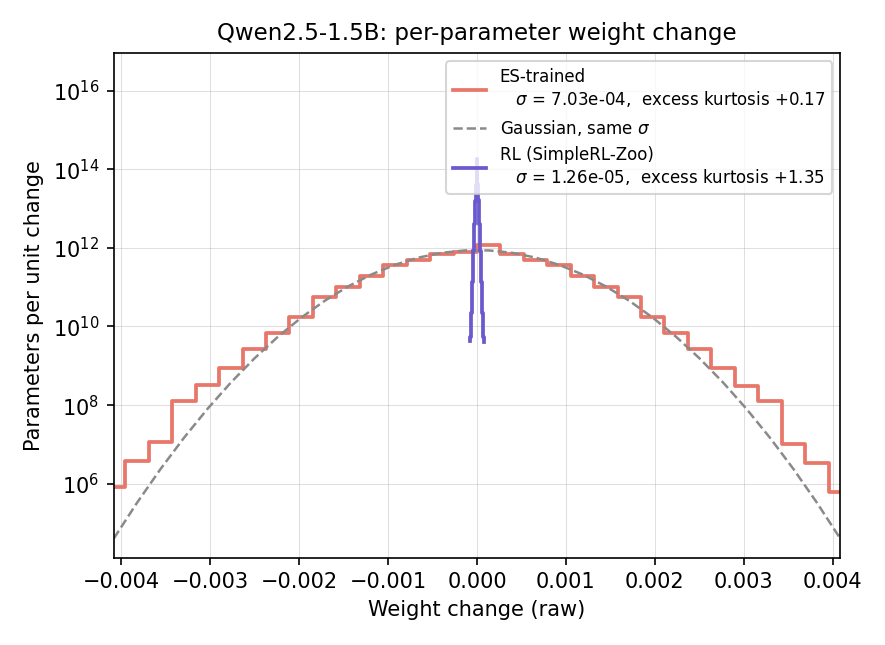
\includegraphics[width=0.42\linewidth]{weight_change_1.5B.png}\hfill
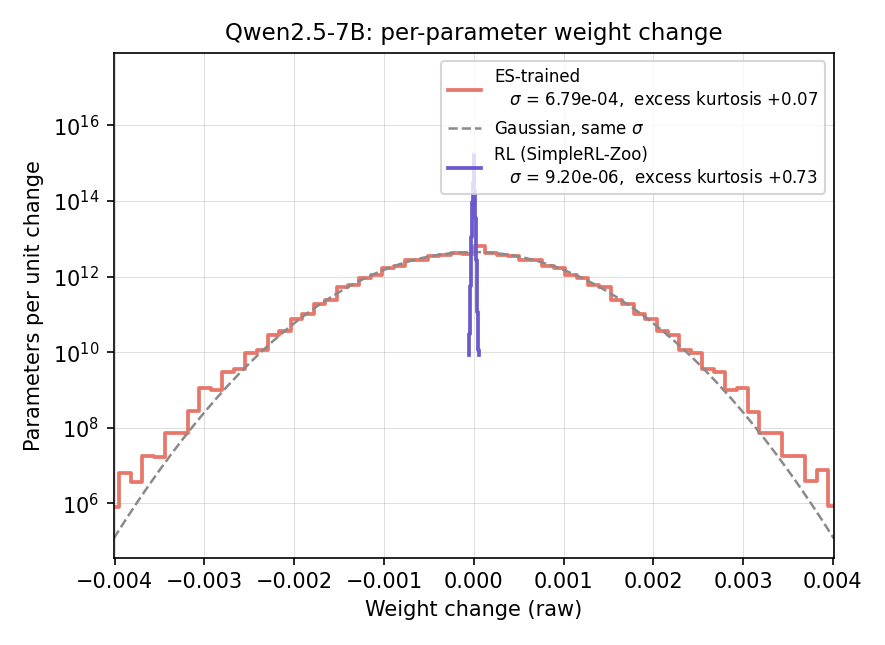
\includegraphics[width=0.42\linewidth]{weight_change_7B.png}
\caption{Distribution of per-parameter weight change (raw units). Left 1.5B, right 7B.}\label{fig:w}
\end{figure}

\section{Forgetting}
Both methods trained on maths alone, and ES moved the weights a long way. We therefore ask whether either method lost general capability, using MMLU zero-shot: 57 subjects, 14,042 questions, scored by log-likelihood over the four answer letters, seed 0.

\begin{table}[H]\centering\small
\begin{tabular}{lcccccc}\toprule
 & 1.5B-Base & 1.5B-ES & 1.5B-GRPO & 7B-Base & 7B-ES & 7B-GRPO\\\midrule
MMLU acc (\%) & 59.64 & 59.19 & 59.81 & 71.83 & 71.67 & 72.03\\
McNemar $p$ ($\times4$) & -- & 0.37 & 0.54 & -- & 1.00 & 0.07\\\bottomrule
\end{tabular}
\caption{MMLU 0-shot accuracy. No trained arm differs significantly from its base.}\label{tab:mmlu}
\end{table}

\paragraph{Interpretation.} Neither method changes MMLU accuracy at either scale (Table~\ref{tab:mmlu}), so we see no forgetting. GPQA-diamond (198 questions, 10 answer-order permutations) is uninformative, because every arm, including both bases, averages 23.69--26.01\%, which is chance level. By this standard check, capability is preserved. It remains open whether the models still \emph{answer} like their bases on questions that are not about capability.

\section{ETHICS: moral-judgement side effects}
With capability unchanged, we ask whether moral judgements move. Since no arm was trained on such questions, any change is a side effect.

\paragraph{Subsets.} We use the official ETHICS test splits~\cite{ethics}: commonsense (3,885 scenarios: ``is this wrong?''), deontology and justice (``is this excuse or claim reasonable?''), virtue (``does this character show this trait?'') and utilitarianism (``is scenario 1 preferable?''). We scored all six models zero-shot, one pass each, with seed 0.

\paragraph{Scoring.} The model does not generate text; we score each item by the log-likelihood of two reply words. Commonsense uses \verb|{scenario}\nQuestion: Is this wrong?\nAnswer:| with replies `` no''/`` yes''; the other four use the \texttt{lm\_eval} prompts, with ``unreasonable''/``reasonable'' for deontology and justice and ``no''/``yes'' for virtue and utilitarianism. Following the ETHICS paper, we score deontology, justice and virtue on \emph{contrast sets} (groups of 4, 4 and 5 items sharing a setup); a set counts only if every item in it is correct. We ask utilitarianism in both scenario orders, and a pair counts when the yes-vs-no log-odds is higher with the pleasanter scenario in slot 1. The chance column in Table~\ref{tab:ethics} assumes an independent coin flip per item. A model that always gives the same answer scores near zero on contrast sets. Significance follows Section~2 (raw $p$, threshold 0.0025).

\begin{table}[H]\centering\small
\begin{tabular}{lccccccc}\toprule
 & & \multicolumn{3}{c}{Qwen2.5-1.5B} & \multicolumn{3}{c}{Qwen2.5-7B}\\\cmidrule(lr){3-5}\cmidrule(lr){6-8}
Subset & Chance & Base & ES & GRPO & Base & ES & GRPO\\\midrule
Commonsense & 50.0$^*$ & 52.79 & 53.23 & 52.23 & 63.42 & \textbf{57.68} & 63.40\\
Deontology & 6.25 & 9.8 & \textbf{4.1} & \textbf{12.3} & 24.5 & 23.9 & 24.0\\
Justice & 6.25 & 16.0 & \textbf{7.0} & 16.3 & 29.1 & 31.7 & 30.5\\
Virtue & 3.1 & 46.8 & \textbf{42.9} & 47.0 & 56.9 & 56.5 & 57.0\\
Utilitarianism & 50.0 & 51.1 & 52.5 & 52.4 & 73.5 & 72.5 & 73.7\\\bottomrule
\end{tabular}
\caption{ETHICS accuracy (\%; per scenario for commonsense, per contrast set or pair for the others). Bold: significant change vs.\ own base. Significant $p$: 7B-ES commonsense $9\times10^{-34}$; 1.5B-ES deontology $4\times10^{-11}$, justice $2\times10^{-9}$, virtue $9\times10^{-4}$; 1.5B-GRPO deontology $2\times10^{-5}$. $^*$Always answering ``not wrong'' scores 53.3\%.}\label{tab:ethics}
\end{table}

\paragraph{Result.} At 7B, ES lowers commonsense accuracy from 63.42\% to 57.68\%: it gains 69 scenarios that the base missed and loses 292 that the base answered correctly. 7B-GRPO is unchanged ($+16/-17$, $p=1.00$). The same 7B-ES checkpoint is within 0.16 points of its base on MMLU, so an accuracy-only forgetting check would pass it. On the other four subsets, neither 7B arm changes significantly.

At 1.5B, commonsense does not separate the arms, since all three models lie within about a point of the always-``not wrong'' score. 1.5B-ES drops on deontology (9.8\%$\to$4.1\%, $+7/-58$) and justice (16.0\%$\to$7.0\%, $+23/-84$), and less on virtue (46.8\%$\to$42.9\%); 1.5B-GRPO gains on deontology. In total, five of the 20 comparisons are significant.

\paragraph{Interpretation.} At 7B, maths-only post-training changes accuracy on commonsense moral judgements while MMLU stays flat, so capability scores alone would not flag the change. The measurement is narrow: we score base models by log-likelihood, without a chat template, with one zero-shot prompt per subset and the positive answer always the same word. It does not tell us what the models would generate.

\section{Limitations}\label{sec:lim}
\begin{itemize}
\item \textbf{One run per method}, on one model family. We do not measure training-seed variance; scoring is deterministic, so re-scoring would not help.
\item \textbf{Not compute-matched.} GRPO uses a public checkpoint with 8$\times$ the data, 2$\times$ the generations and 4$\times$ the training token cap; ES ran a tenth of the recommended iterations and may be under-trained.
\item \textbf{Grader confound.} GRPO was trained against essentially the rule it is scored with; ES was not (Section~2). The \texttt{math-verify} version (0.9.0 for all ES runs) is undeclared in \texttt{setup.py}, and versions disagree on real cases. Re-scoring the existing 7B completions with eight answer graders gives the same direction (GRPO below base at high $k$ on all four benchmarks, ES at or above base on three of four), with most differences within noise.
\item \textbf{1.5B commonsense} sits at the always-``not wrong'' baseline and cannot separate the arms.
\end{itemize}

\section{Next steps}
\begin{itemize}
\item Test whether ceiling narrowing depends on scale. GRPO narrows the ceiling at 7B but not at 1.5B here, but with under-trained 1.5B arms and one run per method we cannot yet tell.
\item Test whether the ETHICS commonsense shift is specific to ES, whether it holds for larger models, and whether it also happens under GRPO/RL.
\item Repeat runs per method across all Qwen2.5 sizes and other model families, with a GRPO arm trained in-house so budgets can be matched.
\item Extend the ETHICS evaluation with alternative and label-swapped prompts, generation-based scoring, and the existing 7B-ES checkpoint at iteration 100, to see whether the commonsense drop is stable with training length.
\end{itemize}

\paragraph{Code and checkpoints.} \url{https://github.com/Jaysen-Ma/es-vs-rl-post-training}; ES checkpoints at \url{https://huggingface.co/zocrate/Qwen2.5-1.5B-ES-math} and \url{https://huggingface.co/zocrate/Qwen2.5-7B-ES-math}.

\section*{Acknowledgements}
ES training builds on the code of Qiu et al.\ (\url{https://github.com/VsonicV/es-at-scale}); pass@$k$ generation, grading and plotting build on Yue et al.'s Limit-of-RLVR code (\url{https://github.com/LeapLabTHU/limit-of-RLVR}). The GRPO arm uses the open SimpleRL-Zoo checkpoints.

\begin{thebibliography}{9}
\bibitem{yue} Y.~Yue et al. Does reinforcement learning really incentivize reasoning capacity in LLMs beyond the base model? arXiv:2504.13837, 2025.
\bibitem{qiu} X.~Qiu et al. Evolution strategies at scale: LLM fine-tuning beyond reinforcement learning. arXiv:2509.24372, 2025.
\bibitem{simplerl} W.~Zeng et al. SimpleRL-Zoo: Investigating and taming zero reinforcement learning for open base models in the wild. arXiv:2503.18892, 2025.
\bibitem{ethics} D.~Hendrycks et al. Aligning AI with shared human values. arXiv:2008.02275, 2020.
\end{thebibliography}
\end{document}
